\section{乱択アルゴリズム}

\begin{frame}[t,fragile]{乱択アルゴリズム(randomized algorithm)}
  \begin{itemize}
    \setlength{\itemsep}{1em}
  \item 実行中に乱数を参照してその値によって振る舞いをかえるアルゴリズム
  \item ラスベガスアルゴリズム
    \begin{itemize}
    \item 乱数の出方によらず常に正しい結果を与えるアルゴリズム
    \item 平均化効果を利用するアルゴリズム:クイックソート
    \end{itemize}
  \item モンテカルロアルゴリズム
    \begin{itemize}
    \item 乱数の出方によっては誤った結果を与えるアルゴリズム
    \item 標本を利用するアルゴリズム:最大カット問題
    \item くじ引き型のアルゴリズム:素数性判定、関数の同一性、行列積の検算
    \item サンプリングアルゴリズム:モンテカルロ積分、マルコフ連鎖モンテカルロ
    \end{itemize}
  \end{itemize}
\end{frame}

\begin{frame}[t,fragile]{乱択クイックソート}
  \begin{itemize}
    \setlength{\itemsep}{1em}
  \item 分割統治法に基づく再帰的なソートアルゴリズム
    \begin{itemize}
      \item 配列の中から要素を一つ選び、それより小さい要素からのみなる集合と大きい要素のみからなる集合の2つに分ける
      \item それぞれの集合をソートし、結合する
    \end{itemize}
    \item ほぼ同じ大きさの集合に分けることができる場合の実行ステップ数$\sim {\cal O}(n \log n)$
    \item 最悪(選んだ要素が常に最大 or 最小値)の場合のステップ数$\sim {\cal O}(n^2)$
    \item 分割に用いる要素を「ランダムに」選ぶ $\Rightarrow$ 平均ステップ数$\sim {\cal O}(n \log n)$
  \end{itemize}
\end{frame}

\begin{frame}[t,fragile]{クイックソート}
  \resizebox{!}{.9\textheight}{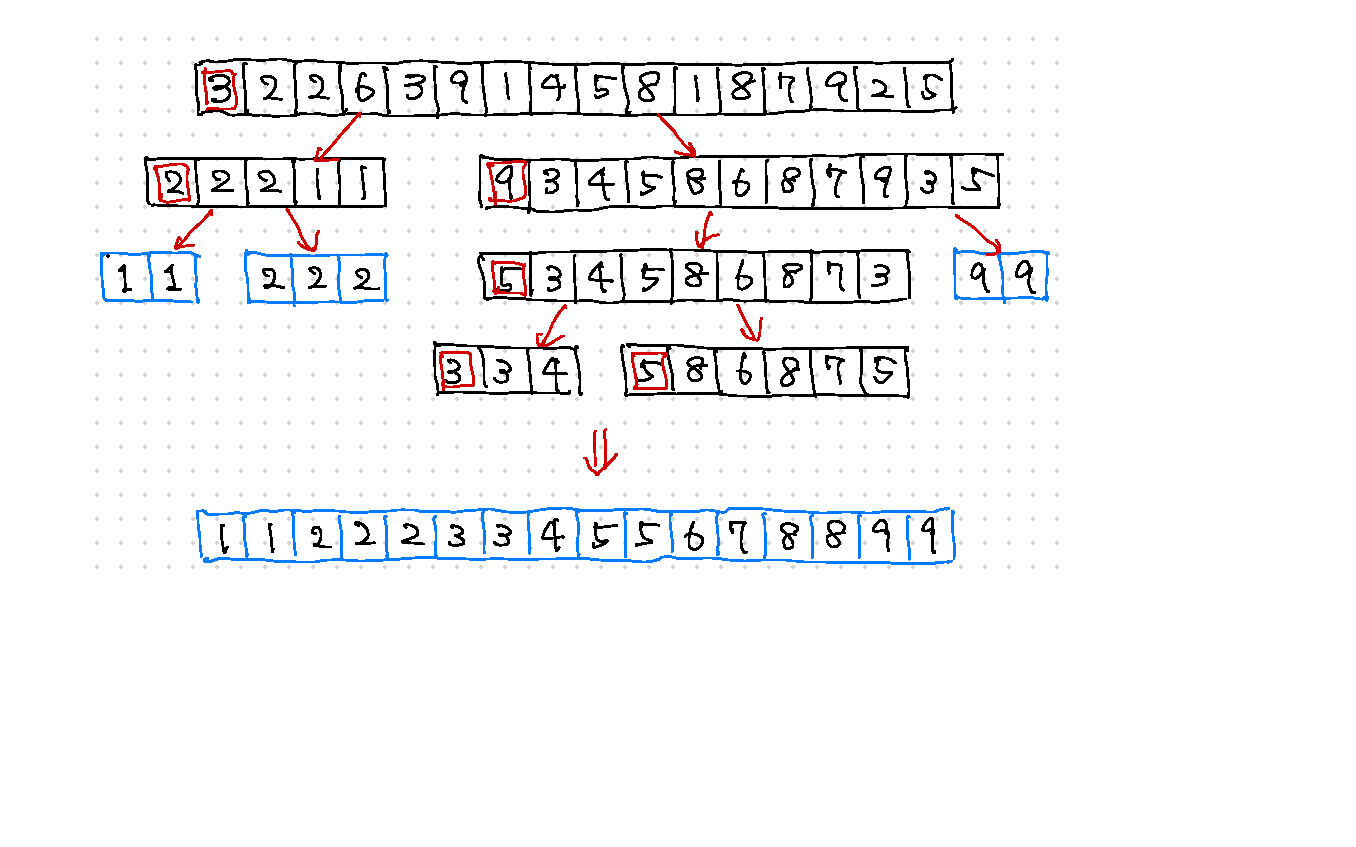
\includegraphics{image/quicksort.pdf}}
\end{frame}

\begin{frame}[t,fragile]{最小カット問題}
  \begin{itemize}
    \setlength{\itemsep}{1em}
  \item 「最小カット (min-cut)」= 連結グラフを二つの部分に分けるために切らなければならない辺(エッジ)の集合のうち、もっとも小さいもの
  \item ``Randomized Min-Cut Algorithm''
    \begin{itemize}
    \item ランダムに辺を一つ選ぶ
    \item 辺の両端の頂点を一つにつぶす(自己ループは取り除く)
    \item 残りの頂点が二つになるまで繰り返す
    \end{itemize}
  \item 上の試行を何回も繰り返して、得られたうちで最小なカットを結果とする
  \item 頂点の数が $n$ のグラフに関して、正解が得られる確率:少なくとも $\frac{2}{n(n-1)}$
  \end{itemize}
\end{frame}

\begin{frame}[t,fragile]{最小カット問題}
  \resizebox{!}{.6\textheight}{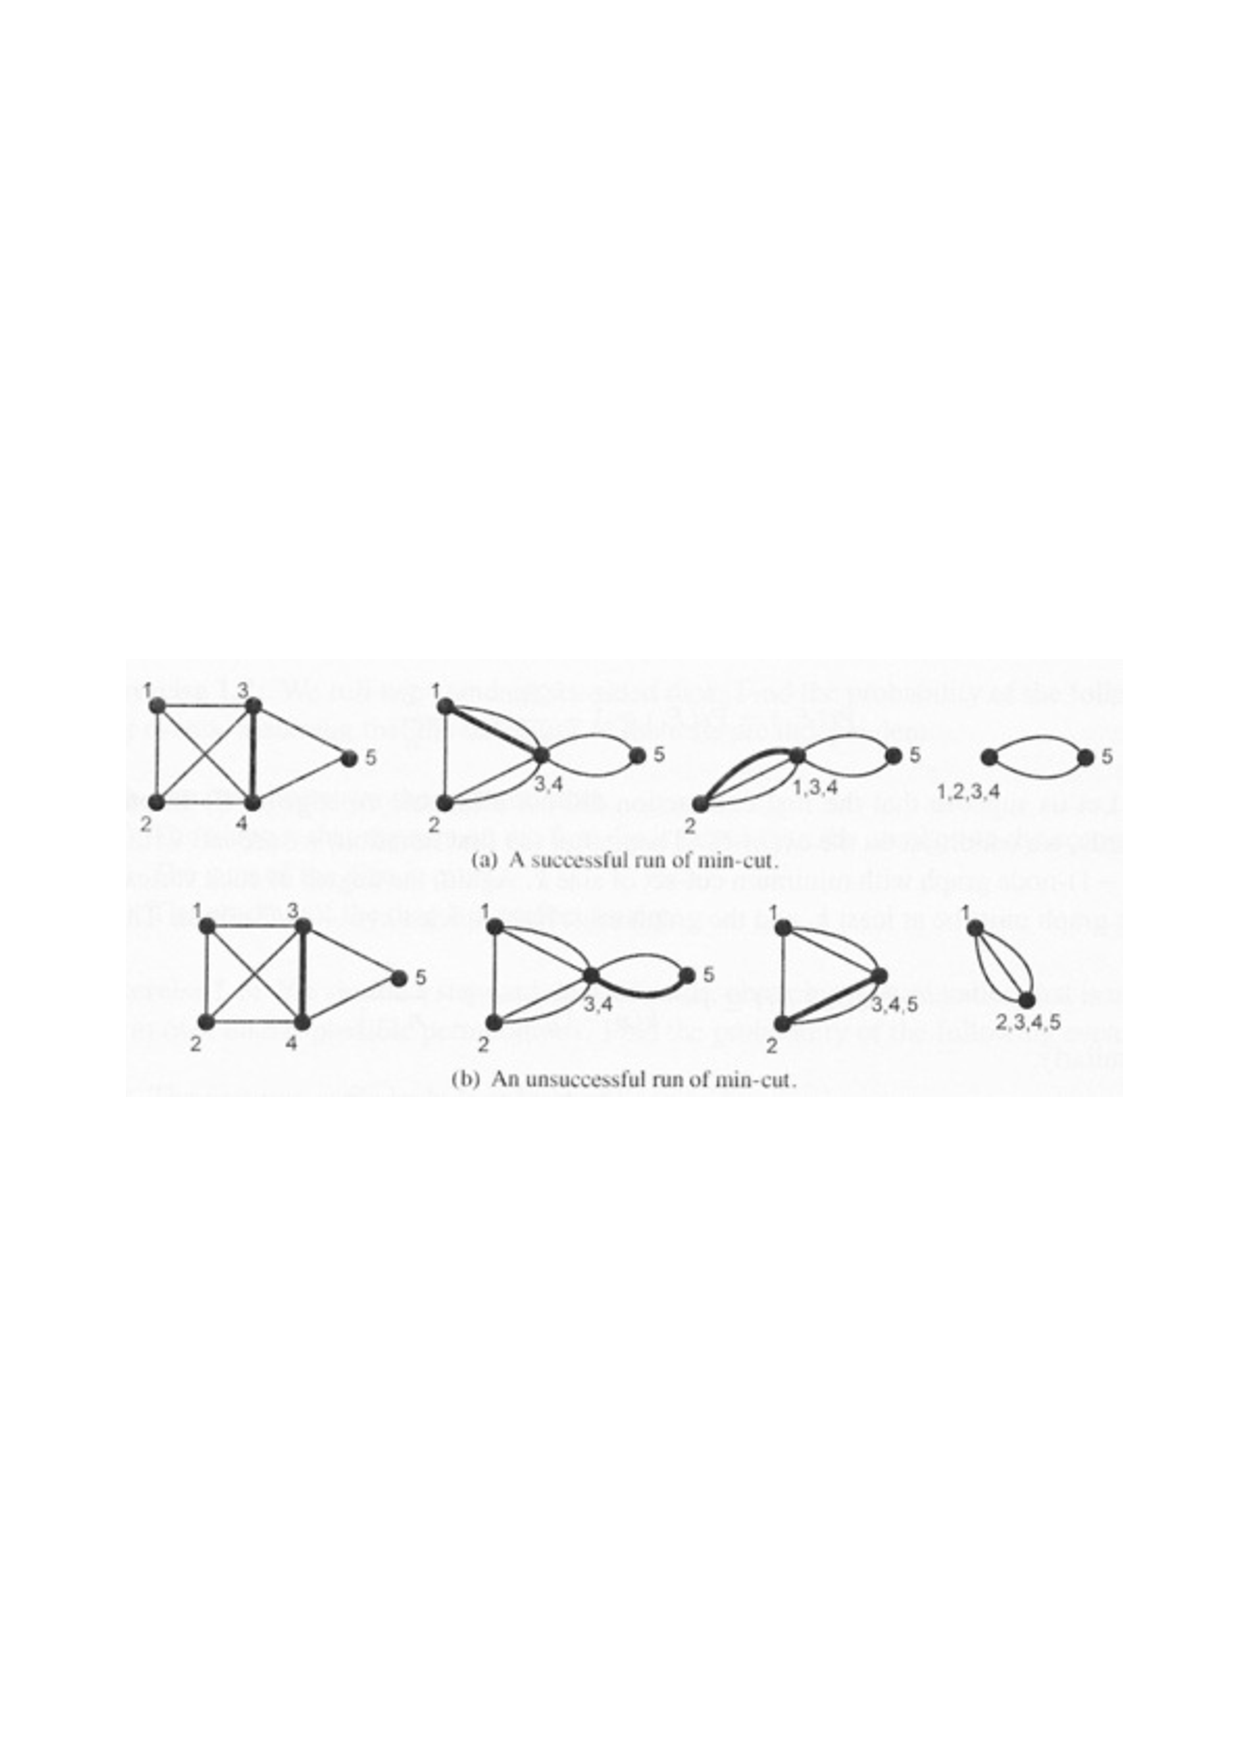
\includegraphics{image/min-cut.pdf}}
\end{frame}
